\exercise{Pitchfork bifurcation}{3}
To explore the pitchfork bifurcation, we consider again a system of the form 
\eq{
\dot{x}=f(x,p)
}
where a physical symmetry stipulates that 
\eq{
f(x,p)=-f(-x,p)
}
\subquestion Use the symmetry condition to show that there is a steady state at $x^*=0$. 
\solution
We can just take the symmetry condition and substitute in the $x=0$. This yields 
\eq{f(0,p)=-f(0,p)}
We can write this also as 
\eq{
2f(0,p)=0
}
which implies 
\eq{
f(0,p)=0 
}
and hence $x=0$ is a steady state regardless of the choice of $p$.

\subquestion
Now use a similar idea to also show 
\eq{
\left. \frac{\partial^n }{\partial x^n} f(x,p) \right|_{x=0} = 0 
}
for all even $n$.

\solution 
Let's see what happens if we differentiate the symmetry condition twice
\eqa{
\frac{\partial^2 }{\partial x^2} f(x,p)&=& -\frac{\partial^2 }{\partial x^2}f(-x,p) \\
\frac{\partial }{\partial x} f'(x,p)&=& +\frac{\partial }{\partial x}f'(-x,p) \\
f''(x,p)&=& -f''(-x,p) 
}
If we substitute $x=0$ this yields
\eq{
f''(0,p)= -f''(0,p) 
}
and hence 
\eq{
f''(0,p)=0.
}
More generally the $n$'th derivative of the symmetry condition is 
\eq{
f^{(n)}(x,p)=-(-1)^n f^{(n)}(x,p)  
}
where we used the superscript $(n)$ to indicate the $n$-th derivative. 
If we now substitute $x=0$ we get 
\eq{
f^{(n)}(0,p)=-(-1)^n f^{(n)}(0,p)  
}
If $n$ is odd this is just the trivial statement 
\eq{
f^{(n)}(0,p)=f^{(n)}(0,p),  
}
but if $n$ is even we get 
\eq{
f^{(n)}(0,p)=-f^{(n)}(0,p),  
}
which implies 
\eq{
f^{(n)}(0,p)=0.  
}

\subquestion
Consider the stability of the steady state at $0$, by setting $x=\delta\ll 1$ and analyzing a suitable Taylor expansion of the dynamics. 
\solution 
This is easier than it sounds. We start with 
\eq{
\dot{delta} = f(\delta,p)
}
Now we Taylor expand $f$ with respect to delta. The first (i.e. zeroth-order) Taylor term is
\eq{
f(0,p) = 0
}
The second term is 
\eq{
f_{\rm x}(0,p)\delta  
}
There is no particular reason why this term should be zero, so we are done. The Taylor expansion that we need is 
\eq{
\dot{delta}=f_{\rm x}(0,p)\delta 
}
which yields the familiar result that the steady state is stable if 
\eq{
f_{\rm x}(0,p)<0.
}

\subquestion
Now assume that the steady state at $x=0$ changes stability at $p^*$ and consider the dynamics close to the bifurcation by setting $p=p^*+\rho$. Taylor expand the dynamics in both $\rho$ and $\delta$ to find the a normal form for the bifurcation. 

\solution 
We start with 
\eq{
\dot{\delta} = f(\delta,p^*+\rho).
}
and Taylor expand we already know
\eq{
f(0,p^*) = 0
}
In addition to these zeroes order Taylor term we can consider derivatives with respect to $x$, derivatives with respect to $p$, and mixed derivatives that contain differentiation with respect to $x$ and $p$. Let's start with the derivatives with respect to $x$.

The first order derivative with respect to $x$ is
\eq{
f_{\rm x}(0,p^*) = 0. 
}
(We actually demanded that this derivative is zero when we said that we want the stability to change at $p^*$). SO we need to go on. The second order with respect to $x$ givens us the Taylor term 
\eq{
f_{\rm xx}(0,p^*) \frac{\delta^2}{2} = 0. 
}
This term is zero because it is an even derivative with respect to $x$. So we go on to the third order 
\eq{
f_{\rm xxx}(0,p^*)\frac{\delta^3}{6} 
}
This is not an even derivative, nor have we assumed that this is zero in our stationarity or bifurcation conditions. So we can stop at this point. 

Now lets consider derivatives with respect to $p$. It turns our that all of these derivatives must be zero. The reason is that if we only differentiate with respect to $p$ we have differentiate 0-times with respect to $x$ and because $0$ is an even number our rule that all even derivatives with respect to $x$ must vanish still holds. 

This leaves us with the mixed derivatives the lowest-order of these is 
\eq{
f_{\rm xp}(0,p^*)\rho\delta 
}
As this is an odd derivative with respect to $x$ and neither our stationarity nor bifurcation conditions stipulate that this should be zero we can assume that this is none zero. All other mixed derivatives have contain a higher order of either $\delta$, $\rho$, or both and are hence negligible. So we are done. 

Our normal form is 
\eq{
\dot{\delta} =  f_{\rm xp}(0,p^*)\rho\delta + f_{\rm xxx}(0,p^*)\frac{\delta^3}{6}. 
}

\subquestion Write the normal form in terms of more convenient variables by defining $\delta$ as the new $x$, $\rho$ as the new $p$ and using $a$ and $b$ for normal form parameters, like we did above. Then compute the steady states and analyze their stability to draw the bifurcation diagram.

\solution
We write the normal form as 
\eq{
\dot{x} =  apx + bx^3. 
}
We can see that there is a steady state at $x^*=0$ and, dividing by $x$, we find two more remaining steady states 
\eq{
x^*=\pm \sqrt{-\frac{a}{b}p}
}
The later steady states exist if $-ap/b>0$, hence we find them at positive values of $p$ if $a/b<0$ and at negative values of $p$ if $a/b>0$.

To determine the stability we consider the derivative 
\eq{
f_{\rm x} = ap +3bx^2
}
Hence the steady state at 0 is stable at for positive $p$ if $a<0$ and at negative $p$ at $a>0$.

Substituting the nontrivial steady states into the stability condition yields
\eq{
f_{\rm x} = ap -3 b \frac{a}{b}p = -2ap
}
Hence the nontrivial states are stable for positive $p$ if $a>0$ and stable for negative $p$ if $a<0$.

We can now draw the bifurcation diagrammes 
\begin{center}
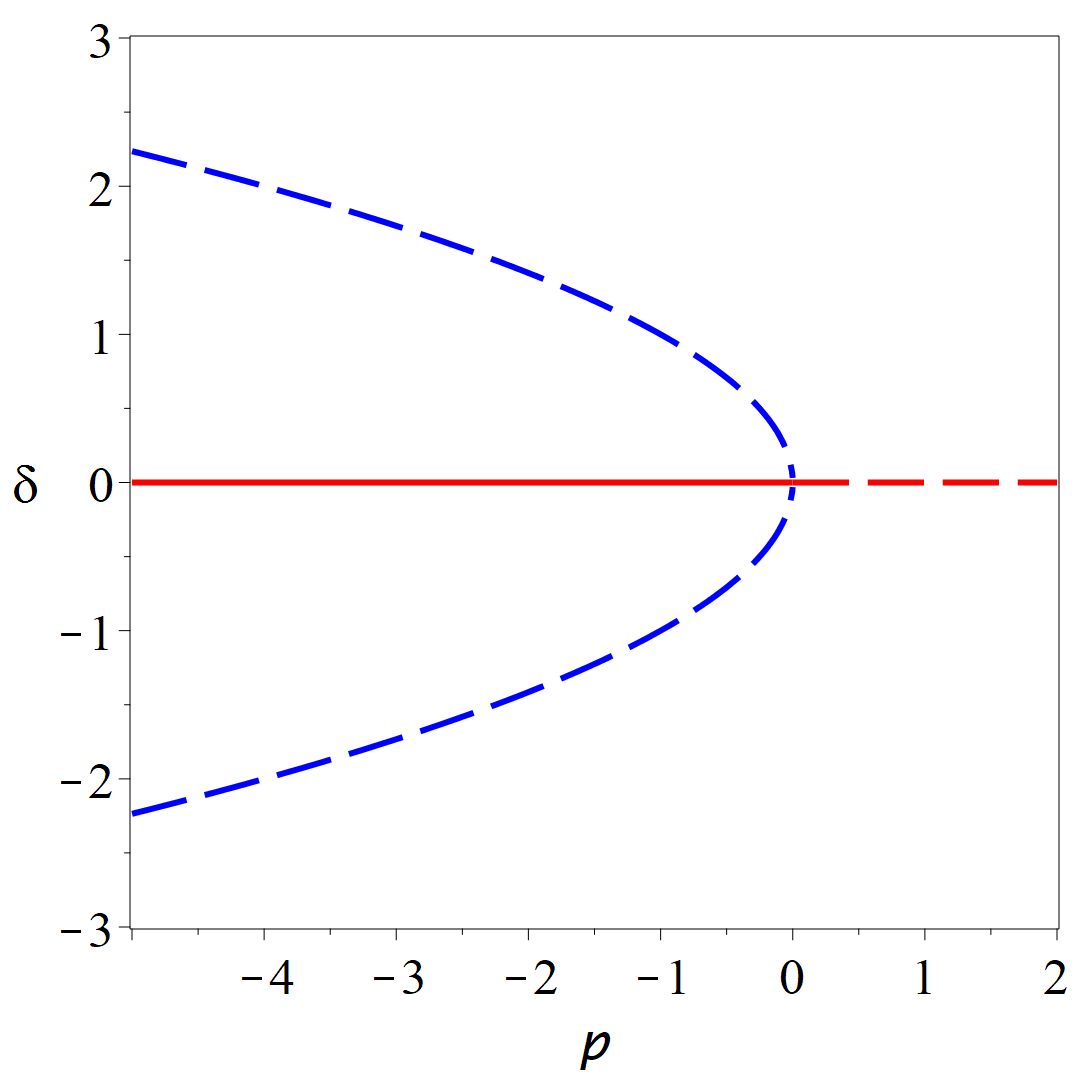
\includegraphics[width=0.45\textwidth]{PitchSub}~~~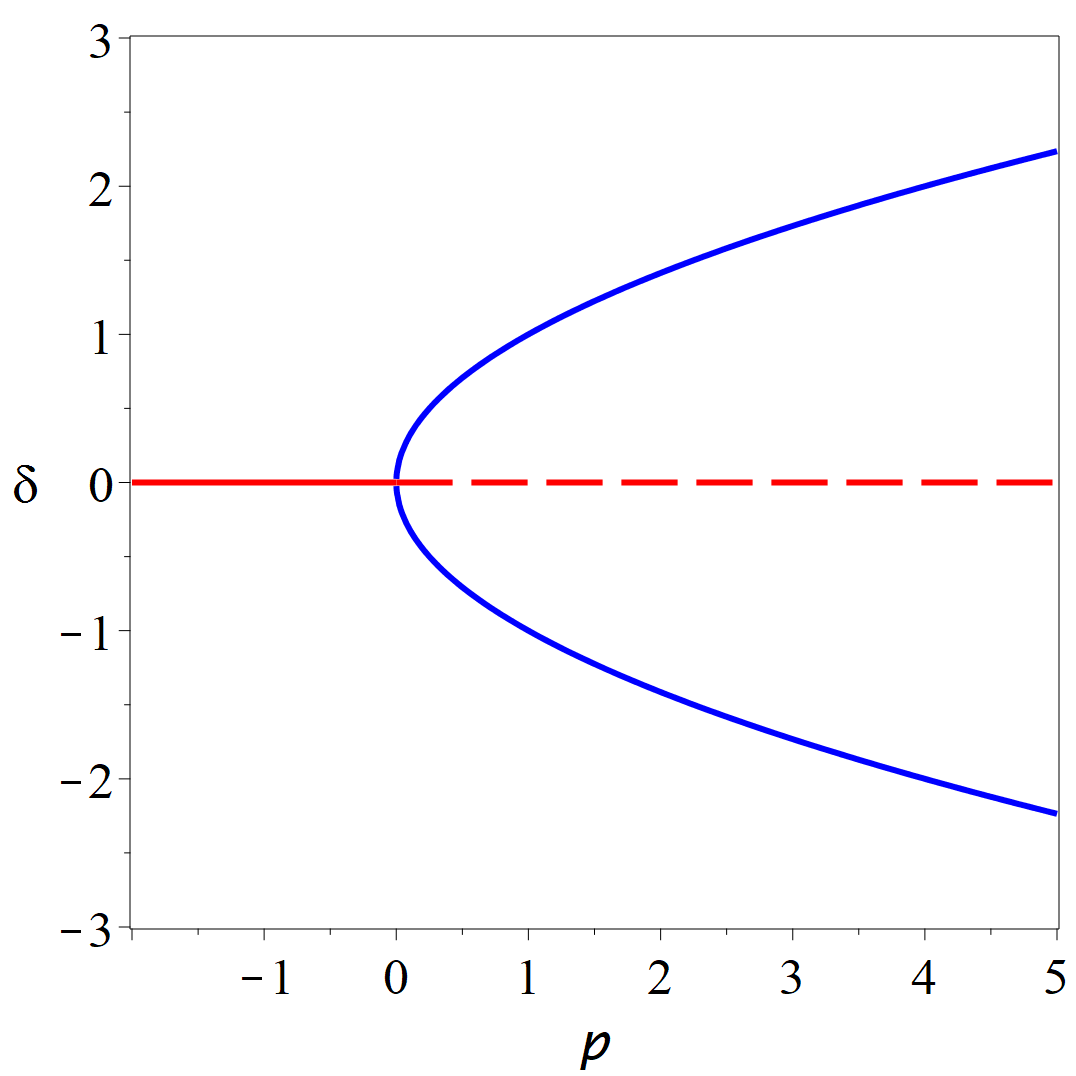
\includegraphics[width=0.45\textwidth]{PitchSuper}
\end{center}
Both of these diagrammes correspond to $a<0$ (trivial steady state is stable for $p<0$). The subcritical case (left) has $b<0$ (nontrivial branches are on the left and unstable) whereas the supercrical case (right) has $b>0$ (nontrivial branches are on the right and stable). 
